\documentclass[11pt,a4paper]{article}

\usepackage[margin=1in]{geometry}
\usepackage{amsmath,amssymb,amsfonts,amsthm}
\usepackage{booktabs}
\usepackage{graphicx}
\usepackage{subcaption}
\usepackage{natbib}
\usepackage{hyperref}
\usepackage{microtype}
\usepackage{tabularx}
\usepackage{xcolor}

\hypersetup{
    colorlinks=true,
    linkcolor=blue!70!black,
    citecolor=blue!70!black,
    urlcolor=blue!70!black
}

\theoremstyle{definition}
\newtheorem{definition}{Definition}
\newtheorem{proposition}{Proposition}
\newtheorem{hypothesis}{Hypothesis}

\title{\textbf{Temporal Regularization in Portfolio Execution: \\ Optimal Holding Horizons Under Signal Decay and Trading Friction}}

\author{
    \textbf{Author Placeholder 1}\thanks{Department of Finance and Economics, Institutional Affiliation Placeholder. Email: author1@institution.edu}
    \and
    \textbf{Author Placeholder 2}\thanks{Department of Computing and Operations Research, Institutional Affiliation Placeholder. Email: author2@institution.edu}
}

\date{\today}

\begin{document}

\maketitle

\begin{abstract}
Quantitative investment strategies that translate periodic predictive signals into target asset weights face a fundamental execution dilemma: continuously rebalancing to follow fresh forecasts maximizes signal responsiveness, but triggers severe portfolio turnover, elevated transaction costs, and concentration in transient estimation noise. Overlapping cohort portfolios---in which capital is staggered across multiple sub-portfolios rolled over horizon $H$---offer an established operational smoothing mechanism. In this paper, we formalize cohort stacking as an architectural \textbf{temporal regularization mechanism} that balances responsiveness to fresh predictive information against execution friction and estimation noise. We derive a stylized analytical expected-utility model over holding horizon $H$, establishing closed-form comparative statics and break-even boundaries for the utility-maximizing horizon within a discrete candidate set $H \in \{1, 2, 4, 8, 13\}$. To evaluate these frontiers without historical empirical distortions, we execute a preregistered synthetic market simulation across 360,000 parameter-seed evaluations under a controlled data-generating process (DGP) where all active cohorts share the single realized market return of each asset per calendar week. All five preregistered comparative static hypotheses are confirmed: the simulated utility-maximizing horizon $H^*$ increases monotonically with transaction costs $c$ (100\% simulation consistency), signal persistence $\rho$ (90\% consistency), observation noise $\sigma_{\text{noise}}$ (100\% consistency), and risk aversion $\gamma$ (100\% consistency), while strong, rapidly decaying alpha favors shorter, more responsive horizons ($H^*=1$; 100\% consistency). Accounting closure holds to machine precision ($|\text{error}| \le 3.144 \times 10^{-17}$), and an audit of the exact-null regime ($\beta=0$) confirms that all horizons tie identically under time-invariant uniform weights ($0.00\text{e}+00$ discrepancy across seven invariants). Finally, we map earlier retrospective empirical post-earnings event studies into this synthetic space, showing that the empirical survival of multi-week cohort stacking was the mathematical consequence of operating a noisy signal under execution friction rather than capturing persistent post-event alpha. We emphasize that Phase~20 is a controlled synthetic investigation and Phases~18--19 provide retrospective empirical motivation; this study does not establish independent prospective or live-trading performance.

\vspace{0.8em}
\noindent \textbf{Keywords:} Portfolio execution, transaction costs, signal decay, holding horizon, temporal regularization, portfolio turnover, overlapping cohorts.

\vspace{0.4em}
\noindent \textbf{JEL Classification Codes:} G11, G12, C61.
\end{abstract}

\newpage

\section{Introduction}
\label{sec:introduction}

A central dilemma in quantitative asset management is managing the tradeoff between forecast freshness and portfolio implementation drag \citep{markowitz1952portfolio, garleanu2013dynamic}. Modern statistical models, machine learning algorithms, and fundamental scoring systems frequently generate refreshed cross-sectional forecasts at high frequencies (e.g., daily or weekly). When an unconstrained optimizer translates these forecasts into target portfolios, the resulting asset weights exhibit severe temporal instability. Rebalancing to track the latest forecast incurs heavy portfolio turnover, elevated transaction costs, and vulnerability to transient estimation noise.

To dampen this churn, quantitative practitioners often employ heuristic execution rules, including trade bands, turnover penalties, or holding-period constraints. Among these, \textbf{overlapping cohort portfolios} (frequently termed ``cohort stacking'') have gained widespread adoption in factor investing and event-driven strategies \citep{jegadeesh1993returns, moskowitz2012time, novymarx2012momentum}. Under cohort stacking with holding horizon $H$, capital is partitioned into $H$ independent sub-portfolios. At each rebalancing date $t$, the oldest sub-portfolio (initiated at date $t-H$) is liquidated, and a fresh sub-portfolio is formed based on the latest signal. The aggregate portfolio is the uniform average of all $H$ currently active cohorts.

While empirically popular, the theoretical mechanisms governing overlapping cohorts are often misunderstood or conflated with predictive alpha. Past literature has frequently attributed the empirical benefits of cohort stacking to the multi-week persistence of the underlying predictive signal, presuming that portfolio gains reflect the capture of prolonged price drift, such as post-earnings announcement drift \citep{bernard1989post}.

In this paper, we demonstrate that cohort stacking operates fundamentally as an \textbf{architectural temporal regularizer}. Even when underlying predictive persistence is negligible or absent, overlapping cohorts mechanically reduce rebalancing turnover by a factor of approximately $1/H$ and diversify idiosyncratic entry-timing variance across active cohorts. However, extending the holding horizon also incurs an inevitable cost: \textbf{alpha dilution}. As cohorts age, decaying predictive signals lose forecasting power, dragging down aggregate portfolio gross returns.

\begin{definition}[\textbf{Optimal Holding Horizon}]
Throughout this paper, the term \emph{optimal horizon} ($H^*$) is strictly defined as the utility-maximizing holding horizon within the discrete candidate set $H \in \{1, 2, 4, 8, 13\}$, under the specified portfolio formation rule, linear transaction-cost model, and mean-variance objective.
\end{definition}

The central research question we address is:
\begin{quote}
\itshape
How does the utility-maximizing cohort holding horizon $H^*$ depend on signal persistence ($\rho$), observation noise ($\sigma_{\mathrm{noise}}$), signal strength ($\beta$), transaction friction ($c$), and portfolio risk aversion ($\gamma$)?
\end{quote}

We address this question through a unified three-part contribution:
\begin{enumerate}
    \item \textbf{Analytical Utility Model}: We construct a stylized expected utility framework formalizing the triad of economic forces---\textbf{alpha dilution}, \textbf{cost amortization}, and \textbf{cross-cohort temporal diversification}---deriving closed-form comparative statics and break-even boundaries.
    \item \textbf{Controlled Synthetic Simulation (Phase 20)}: Under a preregistered simulation design enforcing a single realized asset return per calendar week shared across active cohorts, we evaluate 360,000 parameter-seed instances. We confirm all five primary comparative statics, establish 2D horizon phase diagrams, verify accounting closure to machine precision ($3.144 \times 10^{-17}$), and confirm that time-invariant uniform weights produce an exact mathematical tie across all horizons ($0.00\text{e}+00$ discrepancy).
    \item \textbf{Retrospective Empirical Reconciliation (Phases 18 \& 19)}: We reconcile earlier empirical findings from quarterly corporate earnings announcement portfolios, demonstrating that the empirical survival of multi-week stacking ($H=4$) was an architectural regularizer effect driven by noise suppression and turnover reduction rather than persistent post-earnings drift.
\end{enumerate}

We explicitly delineate the scope of our findings: Phase~20 is a controlled synthetic simulation under stylized linear-Gaussian assumptions; Phases~18 and 19 provide retrospective empirical motivation on historical holdout data (terminating May 15, 2025); and no independent prospective live trading execution is evaluated.


\section{Related Literature and Positioning}
\label{sec:literature}

Our work bridges three distinct strands of financial economics and operations research:

\paragraph{Dynamic Trading with Transaction Costs}
The literature on portfolio execution under trading costs originated with classical proportional and quadratic cost models. \citet{garleanu2013dynamic} established continuous-time dynamic trading rules where the investor trades toward an aim portfolio that linearly averages future expected targets. Overlapping cohort portfolios represent a discrete-time, structural counterpart to continuous aim-portfolio tracking: rather than solving a continuous stochastic control problem, the manager achieves smooth execution by staggering cohort commitments across time.

\paragraph{Overlapping Holding Periods in Factor and Momentum Strategies}
In empirical asset pricing, overlapping holding periods date back to the foundational momentum studies of \citet{jegadeesh1993returns}, who averaged portfolios across overlapping monthly cohorts to boost statistical power and mitigate bid-ask bounce. Similar multi-cohort structures appear in time-series momentum \citep{moskowitz2012time} and post-earnings drift strategies \citep{bernard1989post}. However, these studies primarily treated overlapping cohorts as a backtest smoothing convention rather than an explicit regularizer whose optimal horizon is governed by friction-decay trade-offs.

\paragraph{Model Complexity vs.\ Execution Architecture}
Recent literature in machine learning for finance has investigated whether complex architectures---such as Bayesian neural networks and Parameter-Efficient Fine-Tuning \citep{blundell2015weight, hu2022lora}---or distributed consensus algorithms \citep{papastaikoudis2025distributed} can extract durable market alpha or provide actionable epistemic uncertainty. As documented in our forensic audits (Section~\ref{sec:provenance}), sophisticated predictive signals frequently collapse when subjected to rigorous out-of-sample revalidation. This motivates examining whether operational gains in quantitative portfolios stem from forecast sophistication or from execution architecture.


\section{Analytical Framework of Temporal Regularization}
\label{sec:framework}

\subsection{Mechanics of Overlapping Cohort Portfolios}

Consider a discrete-time investment setting where at each calendar week $t$, a quantitative forecasting model generates an expected return ranking over an asset universe of size $N$. 

Under single-horizon rebalancing ($H=1$), the manager constructs a base portfolio weight vector $w_t^{\text{base}} \in \Delta^{N-1}$ on the probability simplex and rebalances the entire portfolio each period. The one-period rebalancing turnover is:
\begin{equation}
\text{TO}_t^{H=1} = \frac{1}{2} \| w_t^{\text{base}} - w_{t-1}^{\text{base}} \|_1
\end{equation}
Under overlapping cohort stacking with horizon $H \in \{1, 2, \dots\}$, capital is partitioned equally across $H$ sub-portfolios. At period $t$, the cohort entered at $t-H$ is liquidated, and a fresh cohort with target weights $w_t^{\text{base}}$ is initiated. The aggregate portfolio weight vector $w_t^H$ is the uniform average:
\begin{equation}
w_t^H = \frac{1}{H} \sum_{k=0}^{H-1} w_{t-k}^{\text{base}}
\end{equation}
Assuming stationary rebalancing dynamics, the turnover of the aggregate portfolio scales inversely with the horizon:
\begin{equation}
\text{TO}_t^H = \frac{1}{2} \| w_t^H - w_{t-1}^H \|_1 = \frac{1}{2H} \| w_t^{\text{base}} - w_{t-H}^{\text{base}} \|_1 \approx \frac{\text{TO}_0}{H}
\end{equation}
where $\text{TO}_0$ denotes the characteristic one-period base turnover. Figure~\ref{fig:architecture} illustrates this conceptual architecture.

\begin{figure}[t]
\centering
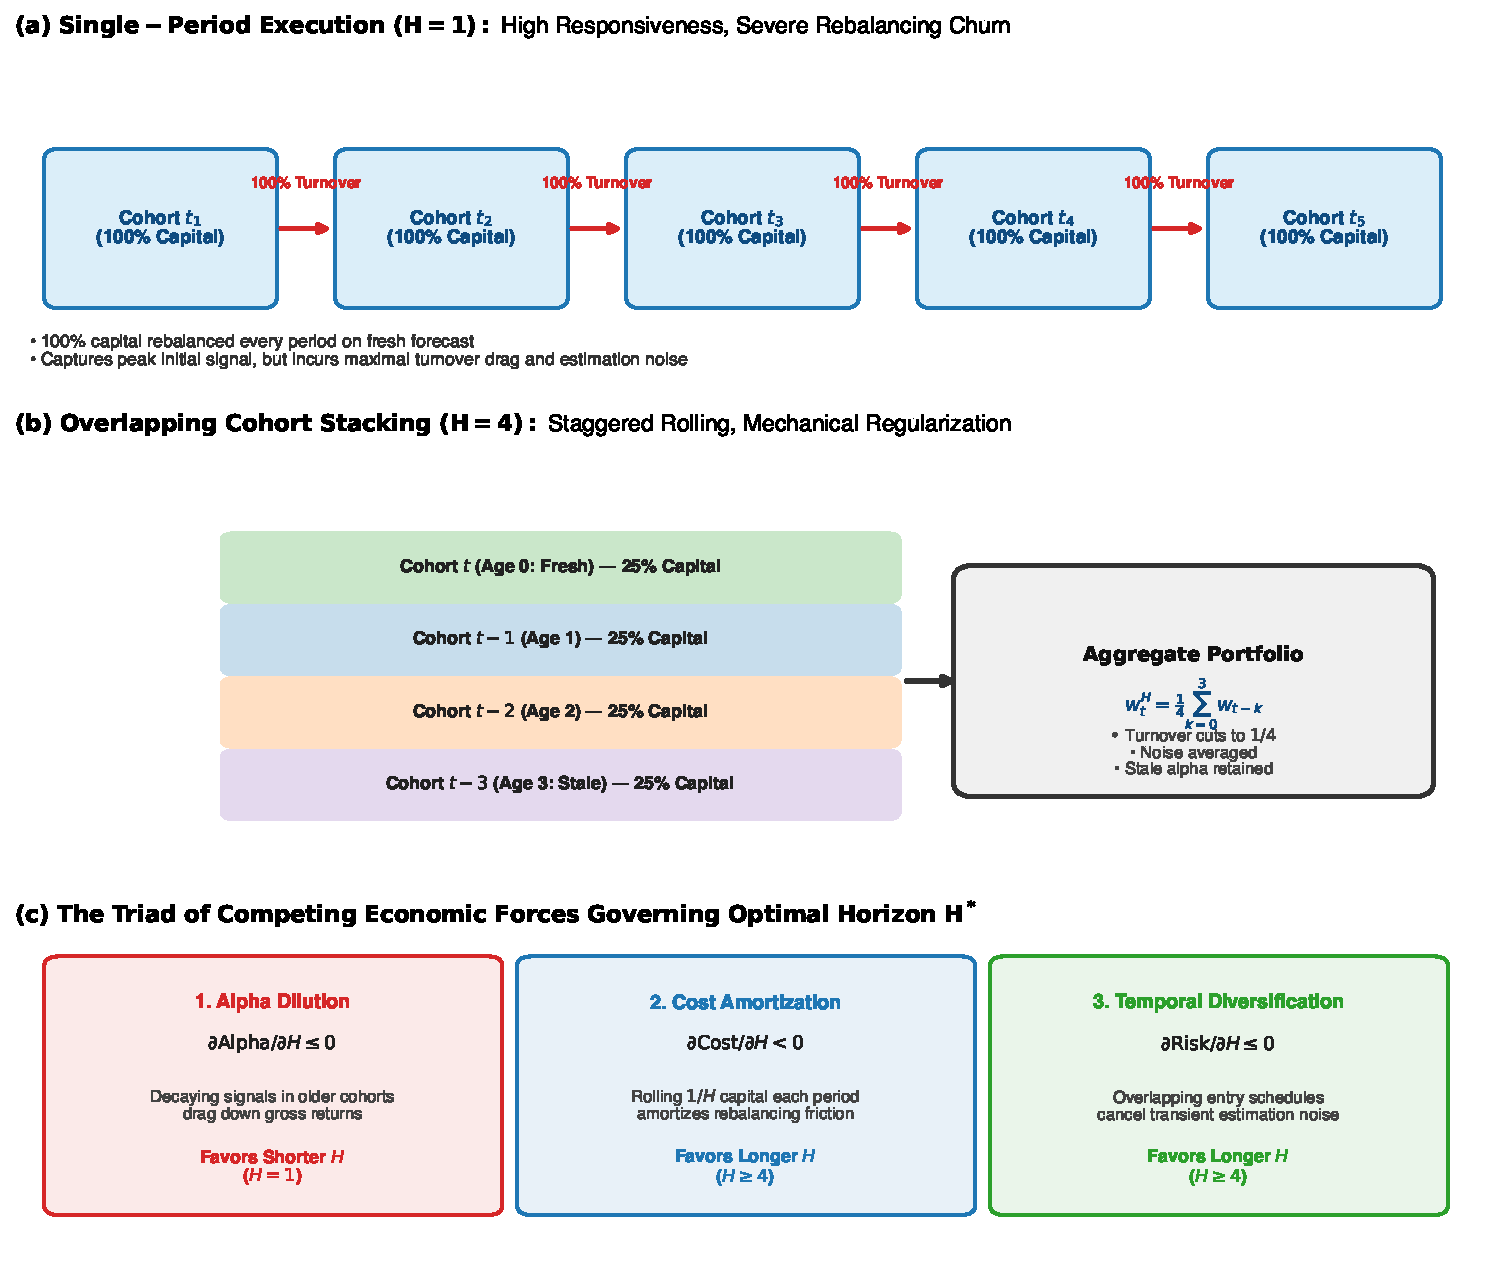
\includegraphics[width=0.95\textwidth]{figures/fig1_temporal_regularization_architecture.pdf}
\caption{\textbf{Conceptual Architecture of Temporal Regularization.} (a) Single-period execution ($H=1$) rebalances 100\% of capital each week, incurring high turnover and full noise exposure. (b) Overlapping cohort stacking ($H=4$) partitions capital across four staggered sub-portfolios, cutting turnover to $1/4$ and averaging cross-cohort weights. (c) The triad of competing economic forces governing optimal horizon selection $H^*$.}
\label{fig:architecture}
\end{figure}

\subsection{Stylized Expected Utility Model}

Let predictive signal quality decay geometrically with holding age $k \ge 0$:
\begin{equation}
\mu_k = \mu_0 \rho^k = \mu_0 e^{-k / \tau}
\end{equation}
where $\mu_0 \ge 0$ is initial gross alpha at entry age $k=0$, $\rho \in [0, 1)$ is the one-period signal persistence parameter, $\tau = -1/\ln(\rho)$ is the decay time, and $\tau_{1/2} = \ln(0.5)/\ln(\rho)$ is the signal half-life.

The expected gross alpha captured by an aggregate portfolio of horizon $H$ is the average across all active cohort ages:
\begin{equation}
\bar{r}_{\text{gross}}(H) = \frac{1}{H} \sum_{k=0}^{H-1} \mu_0 \rho^k = 
\begin{cases} 
\mu_0 \frac{1 - \rho^H}{H(1 - \rho)}, & \text{if } \rho < 1 \\ 
\mu_0, & \text{if } \rho = 1 
\end{cases}
\end{equation}
The portfolio incurs linear transaction friction with cost rate $c$ per unit of traded turnover:
\begin{equation}
\text{Cost}(H) = c \cdot \text{TO}(H) \approx \frac{c \cdot \text{TO}_0}{H}
\end{equation}
Aggregate portfolio variance decomposes into market-wide systematic variance $\sigma_0^2$ and cohort-specific estimation/timing variance $\sigma_1^2$. Because active cohorts are initiated at staggered dates with independent estimation noise, cross-cohort averaging diversifies cohort-specific variance:
\begin{equation}
\sigma^2(H) \approx \sigma_0^2 + \frac{\sigma_1^2}{H}
\end{equation}
Combining these components under a mean-variance utility objective with risk aversion parameter $\gamma \ge 0$, we define stylized expected utility:
\begin{equation}
U(H) = \mu_0 \frac{1 - \rho^H}{H(1 - \rho)} - \frac{c \cdot \text{TO}_0}{H} - \frac{1}{2}\gamma \left(\sigma_0^2 + \frac{\sigma_1^2}{H}\right)
\label{eq:utility}
\end{equation}

\subsection{The Triad of Competing Economic Forces}

Differentiating utility with respect to horizon $H$ highlights three fundamental forces:
\begin{enumerate}
    \item \textbf{Alpha Dilution ($\partial \text{Alpha}/\partial H \le 0$)}: Older cohorts retain stale signals, diluting fresh predictive information. For any $\rho < 1$, alpha dilution strictly penalizes longer horizons and favors $H=1$.
    \item \textbf{Cost Amortization ($\partial \text{Cost}/\partial H < 0$)}: Rolling $1/H$ of the portfolio amortizes turnover friction proportionally to $1/H$, strictly favoring longer horizons whenever $\text{TO}_0 > 0$ and $c > 0$.
    \item \textbf{Temporal Diversification ($\partial \text{Risk}/\partial H \le 0$)}: Overlapping cohorts average independent estimation noise and entry-timing variance, reducing portfolio variance and favoring longer horizons whenever $\sigma_1^2 > 0$ and $\gamma > 0$.
\end{enumerate}

\paragraph{Boundary Behavior}
When signals are purely transient ($\rho = 0$), $\bar{r}_{\text{gross}}(H) = \mu_0 / H$, causing alpha to collapse rapidly. In contrast, under permanent signals ($\rho \to 1$), $\bar{r}_{\text{gross}}(H) = \mu_0$ and alpha dilution vanishes. Crucially, when rebalancing churn is identically zero ($\text{TO}_0 = 0$ and $\sigma_1^2 = 0$, as in time-invariant equal weighting), $U(H) = -\frac{1}{2}\gamma \sigma_0^2$ for all $H$, producing an exact tie. Stacking gains emerge exclusively when base allocations churn across periods.


\section{Analytical Comparative Statics and Break-Even Frontiers}
\label{sec:comparative_statics}

To evaluate optimal horizon selection, we analyze the utility differential relative to the single-period baseline $H=1$:
\begin{equation}
\Delta U(H, 1) = U(H) - U(1) = \mu_0 \left[ \frac{1 - \rho^H}{H(1 - \rho)} - 1 \right] + c \cdot \text{TO}_0 \left(1 - \frac{1}{H}\right) + \frac{1}{2}\gamma \sigma_1^2 \left(1 - \frac{1}{H}\right)
\end{equation}
Factoring out $(1 - 1/H)$:
\begin{equation}
\Delta U(H, 1) = \left(1 - \frac{1}{H}\right) \left\{ c \cdot \text{TO}_0 + \frac{1}{2}\gamma \sigma_1^2 - \mu_0 \Lambda(H, \rho) \right\}
\end{equation}
where the effective information decay factor is defined as:
\begin{equation}
\Lambda(H, \rho) \equiv \frac{1 - \frac{1 - \rho^H}{H(1 - \rho)}}{1 - 1/H}
\end{equation}
From this formulation, we analytically derive five primary comparative statics (Figure~\ref{fig:tradeoff}):

\begin{figure}[t]
\centering
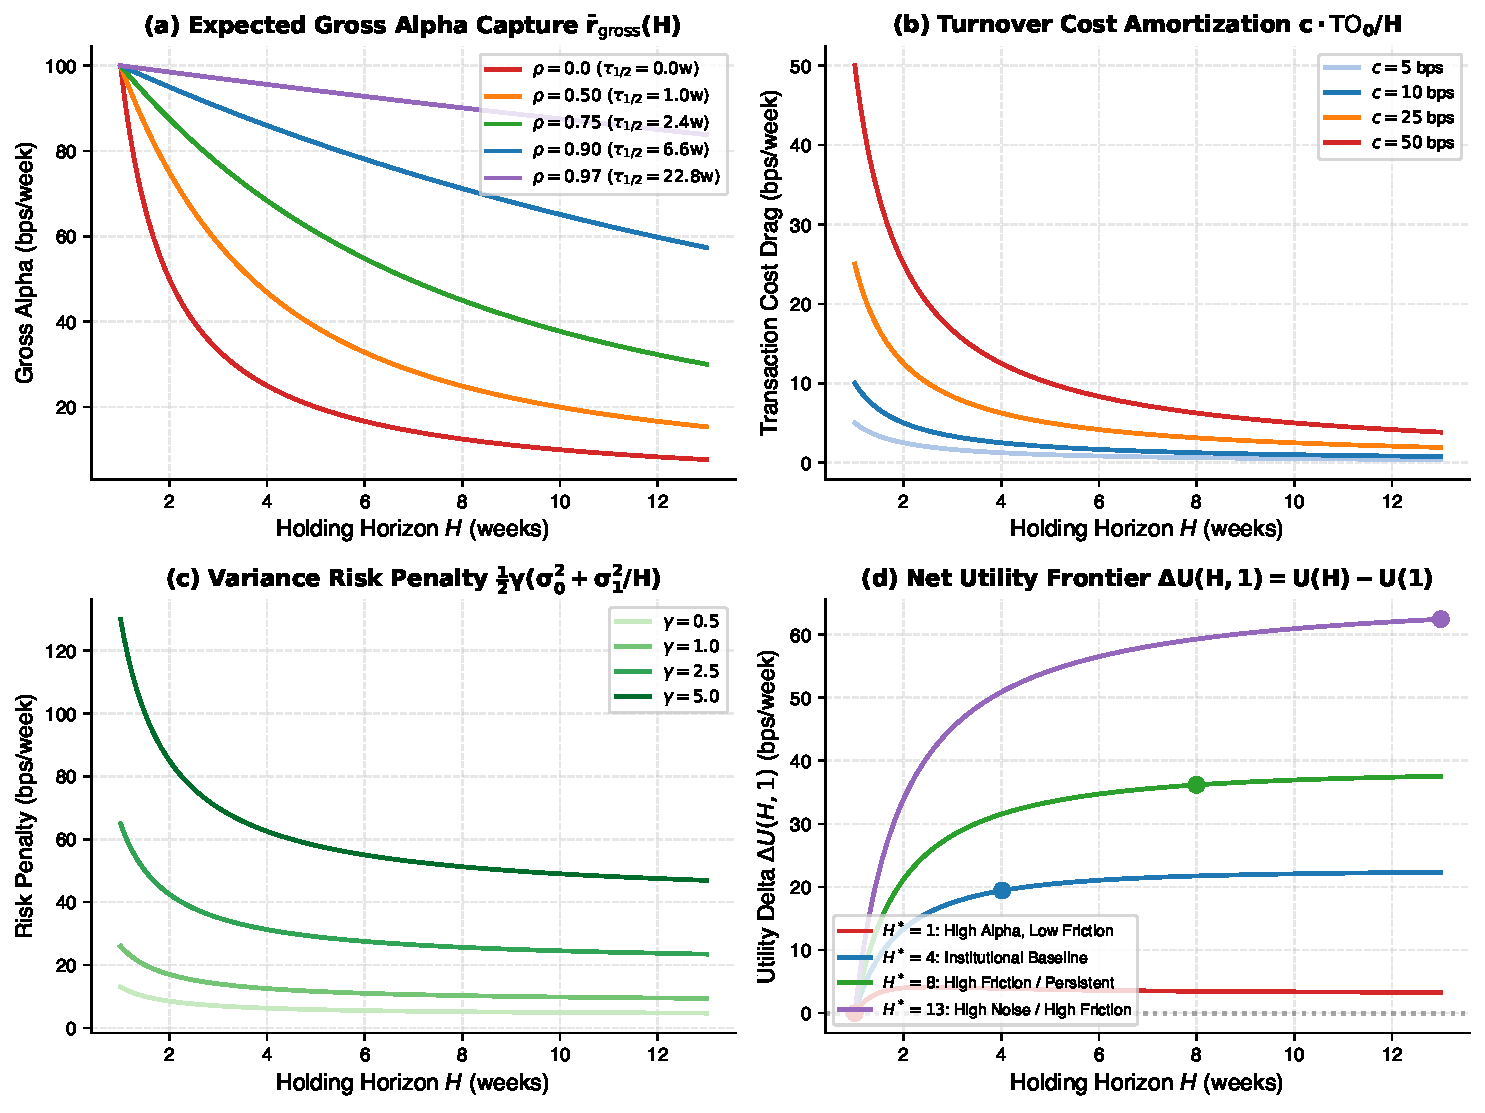
\includegraphics[width=0.95\textwidth]{figures/fig2_analytical_tradeoff.pdf}
\caption{\textbf{Analytical Expected Utility Tradeoff and Comparative Statics.} (a) Gross alpha capture $\bar{r}_{\text{gross}}(H)$ under varying persistence $\rho$. (b) Turnover cost amortization $c \cdot \text{TO}_0 / H$ across cost rates $c$. (c) Variance penalty reduction across risk aversion $\gamma$. (d) Resulting net utility frontier $\Delta U(H, 1)$, illustrating the monotonic shift in optimal horizon $H^*$ across parameter regimes.}
\label{fig:tradeoff}
\end{figure}

\begin{proposition}[\textbf{Cost Monotonicity, H1}]
For any horizon $H > 1$ and baseline turnover $\text{TO}_0 > 0$:
\begin{equation}
\frac{\partial \Delta U(H, 1)}{\partial c} = \text{TO}_0 \left(1 - \frac{1}{H}\right) > 0
\end{equation}
Higher transaction friction increases the marginal value of turnover reduction, weakly increasing the utility-maximizing horizon: $\partial H^* / \partial c \ge 0$.
\end{proposition}

\begin{proposition}[\textbf{Persistence Monotonicity, H2}]
For any active signal ($\mu_0 > 0$), differentiating alpha capture with respect to persistence $\rho$ yields:
\begin{equation}
\frac{\partial}{\partial \rho}\left[ \frac{1 - \rho^H}{1 - \rho} \right] = \frac{1 - H\rho^{H-1} + (H-1)\rho^H}{(1 - \rho)^2} > 0 \quad (\forall H > 1, \rho \in [0, 1))
\end{equation}
Because $\partial \Lambda(H, \rho) / \partial \rho < 0$, higher persistence slows alpha dilution, expanding the parameter region where cost and risk savings dominate: $\partial H^* / \partial \rho \ge 0$.
\end{proposition}

\begin{proposition}[\textbf{Short-Lived Alpha Reversal, H3}]
In the frictionless limit ($c = 0$) under transient signals ($\rho = 0$):
\begin{equation}
\Delta U(H, 1)\big|_{\rho=0, c=0} = \left(1 - \frac{1}{H}\right) \left[ \frac{1}{2}\gamma \sigma_1^2 - \mu_0 \right]
\end{equation}
For unconstrained alpha ($\mu_0 > \frac{1}{2}\gamma \sigma_1^2$), this differential is strictly negative for all $H > 1$, establishing $H^* = 1$. Furthermore, for any $\rho < 1$:
\begin{equation}
\frac{\partial \Delta U(H, 1)}{\partial \mu_0} = \frac{1 - \rho^H}{H(1 - \rho)} - 1 \le 0
\end{equation}
As signal strength $\mu_0$ increases, the absolute penalty of holding stale cohorts scales up linearly, shifting preference toward shorter, more responsive horizons.
\end{proposition}

\begin{proposition}[\textbf{Noise Regularization, H4}]
When observed signals contain additive ranking error $\hat{s} = s + \sigma_{\text{noise}}\eta$, initial alpha scales as $\mu_0 \propto 1 / \sqrt{1 + \sigma_{\text{noise}}^2}$. As noise increases, alpha dilution weakens while cross-cohort noise cancellation retains value: $\partial H^* / \partial \sigma_{\text{noise}} \ge 0$.
\end{proposition}

\begin{proposition}[\textbf{Risk Aversion Preference, H5}]
\begin{equation}
\frac{\partial \Delta U(H, 1)}{\partial \gamma} = \frac{1}{2}\sigma_1^2 \left(1 - \frac{1}{H}\right) > 0 \quad (\forall H > 1, \sigma_1^2 > 0)
\end{equation}
Higher risk aversion increases the utility penalty assigned to portfolio variance, expanding preference for the diversification offered by overlapping cohorts: $\partial H^* / \partial \gamma \ge 0$.
\end{proposition}

\subsection{Closed-Form Break-Even Boundaries}
Setting $\Delta U(H, 1) = 0$ yields closed-form break-even frontiers:
\begin{equation}
c^*(H) = \frac{\mu_0 \Lambda(H, \rho) - \frac{1}{2}\gamma \sigma_1^2}{\text{TO}_0}
\end{equation}
If actual execution cost $c > c^*(H)$, horizon $H$ delivers strictly higher net utility than $H=1$. Similarly, the break-even alpha boundary is:
\begin{equation}
\mu_0^*(H) = \frac{c \cdot \text{TO}_0 + \frac{1}{2}\gamma \sigma_1^2}{\Lambda(H, \rho)}
\end{equation}


\section{Controlled Synthetic Experiment Design (Phase 20)}
\label{sec:design}

To test these comparative statics empirically without reliance on historical market anomalies, we implemented a controlled synthetic market simulation.

\subsection{Data-Generating Process (DGP)}

\paragraph{Asset Universe and Evaluation Horizon}
The simulation models $N = 30$ assets across $T = 156$ calendar weeks (3 years of weekly rebalancing) following a 52-week initialization burn-in. Horizons were frozen at $H \in \{1, 2, 4, 8, 13\}$.

\paragraph{Latent Information Process}
At each calendar week $t$, each asset $i$ receives an independent latent predictive factor $s_{i,t} \sim \mathcal{N}(0, 1)$.

\paragraph{Single Realized Market Return Invariance}
Crucially, to eliminate cohort-specific return noise or oracle leaks, each asset has \textbf{exactly one realized market return per calendar week}, shared by every active cohort holding that asset:
\begin{equation}
R_{u, i} = \sum_{k=0}^{K} \beta \rho^k s_{i, u-k} + \epsilon_{\text{mkt}, u} + \xi_{u, i}
\label{eq:dgp_return}
\end{equation}
where $K = 52$ truncates the latent history, $\beta$ governs signal magnitude, $\epsilon_{\text{mkt}, u} \sim \mathcal{N}(0, \sigma_{\text{mkt}}^2)$ with $\sigma_{\text{mkt}} = 0.02$ (2\% weekly market volatility) is a shared systematic factor shock, and $\xi_{u, i} \sim \mathcal{N}(0, \sigma_{\text{idio}}^2)$ with $\sigma_{\text{idio}} = 0.04$ (4\% weekly idiosyncratic volatility) is an asset-specific calendar return shock.

\paragraph{Finite-Memory Truncation Disclosure}
For the highest persistence level ($\rho = 0.97$), $0.97^{52} \approx 0.2032$. Thus, the 52-week truncation leaves approximately $20\%$ of latent signal weight unmodeled. The $\rho = 0.97$ case is therefore an explicitly finite-memory approximation rather than an asymptotic infinite-history AR(1) process.

\paragraph{Noisy Ranking Signals}
At entry week $t$, portfolio weights are formed by ranking assets on noisy observed signals:
\begin{equation}
\hat{s}_{i,t} = s_{i,t} + \sigma_{\text{noise}} \eta_{i,t}, \quad \eta_{i,t} \sim \mathcal{N}(0, 1)
\end{equation}

\paragraph{Exact-Null Baseline}
At $\beta = 0.000$, ranking signals are deactivated, and base portfolio weights are set to uniform equal weighting ($w_{i,t} = 1/N$).

\subsection{Preregistered Simulation Matrix \& Invariants}
As detailed in Table~\ref{tab:simulation_design}, the simulation evaluates a complete factorial design spanning 360,000 portfolio-horizon evaluations across 30 independent seeds ($S \in \{200001, \dots, 200030\}$).

Numerical closure was audited against the algebraic identity:
\begin{equation}
\Delta U(H_A, H_B) = (\bar{r}_{\text{gross}, A} - \bar{r}_{\text{gross}, B}) - c(\overline{\text{TO}}_A - \overline{\text{TO}}_B) - \frac{1}{2}\gamma(\text{Var}(r_{\text{net}, A}) - \text{Var}(r_{\text{net}, B}))
\end{equation}
with required tolerance $|\text{error}| < 10^{-12}$. Statistical ties across seeds were evaluated using paired two-sided $t$-tests ($\alpha = 0.05$).

\begin{table}[t]
\centering
\small
\caption{\textbf{Phase 20 Synthetic Factorial Simulation Design and Audit Summary.} Complete parameter specification and machine-precision numerical audit across 360,000 evaluations. All active cohorts share a single realized market return per calendar week for each asset.}
\label{tab:simulation_design}
\resizebox{\textwidth}{!}{%
\begin{tabular}{lll}
\hline
\textbf{Dimension / Parameter} & \textbf{Specification / Value} & \textbf{Methodological Role / Audit Bound} \\
\hline
Asset Cross-Section ($N$) & 30 assets & Controlled synthetic equities universe \\
Evaluation Calendar ($T$) & 156 calendar weeks & 3 years of weekly portfolio rebalancing \\
Latent History Truncation ($K$) & 52 weeks & Truncation bound: $0.97^{52} \approx 0.2032$ (finite-memory AR(1)) \\
Market Factor Volatility ($\sigma_{\text{mkt}}$) & 0.02 (2\% weekly) & Common systematic calendar return shock \\
Idiosyncratic Volatility ($\sigma_{\text{idio}}$) & 0.04 (4\% weekly) & Asset-specific calendar return shock \\
Simulation Seeds & 30 seeds ($200001$--$200030$) & Independent synthetic market realizations \\
Candidate Holding Horizons ($H$) & $\{1, 2, 4, 8, 13\}$ weeks & Frozen discrete candidate set (5 levels) \\
Signal Strength ($\beta$) & $\{0.000, 0.005, 0.010, 0.020\}$ & Latent factor return loading (4 levels) \\
Weekly Persistence ($\rho$) & $\{0.0, 0.25, 0.50, 0.75, 0.90, 0.97\}$ & Implied half-life $\tau_{1/2} \in [0.0, 22.8]$ weeks (6 levels) \\
Signal Observation Noise ($\sigma_{\text{noise}}$) & $\{0.0, 0.5, 1.0, 2.0\}$ & Additive Gaussian ranking noise (4 levels) \\
Transaction Cost Rate ($c$) & $\{0, 5, 10, 25, 50\}$ bps & Linear proportional turnover friction (5 levels) \\
Risk Aversion ($\gamma$) & $\{0.0, 0.5, 1.0, 2.5, 5.0\}$ & Mean-variance utility objective weight (5 levels) \\
\hline
\textbf{Total Factorial Evaluations} & \textbf{360,000 evaluations} & $4 \times 6 \times 4 \times 5 \times 5 \times 5 \times 30$ full matrix \\
Pairwise Comparisons vs $H=1$ & 288,000 comparisons & Pairwise accounting and paired $t$-test tie audit \\
Accounting Closure Max Error & $\mathbf{3.144 \times 10^{-17}}$ & Algebraic identity verified ($|\text{error}| \ll 10^{-12}$) \\
Exact-Null ($\beta=0$) Discrepancy & $\mathbf{0.00\text{e}+00}$ & 7 invariants pass with zero error (100\% \texttt{Tie\_1-2-4-8-13}) \\
Preregistered Adjudication & \textbf{Outcome A} & Frontier confirmed; closure verified; 5/5 hypotheses passed \\
\hline
\end{tabular}%
}
\end{table}


\section{Synthetic Simulation Results}
\label{sec:results}

\subsection{Confirmation of Comparative Static Hypotheses}

Across all 360,000 evaluations, the synthetic simulation confirmed all five preregistered comparative static hypotheses (Table~\ref{tab:comparative_statics}):

\begin{table}[t]
\centering
\small
\caption{\textbf{Phase 20 Primary Comparative Statics Confirmation.} Consistency reflects the proportion of pairwise parameter transitions across 360,000 evaluations conforming to the theoretical prediction. Hypothesis H2 is evaluated on active signals ($\beta > 0$). All evaluations satisfy accounting closure to machine precision ($|\text{error}| \le 3.144 \times 10^{-17}$).}
\label{tab:comparative_statics}
\resizebox{\textwidth}{!}{%
\begin{tabular}{llccc}
\hline
\textbf{Hypothesis} & \textbf{Economic Mechanism} & \textbf{Predicted Direction} & \textbf{Simulation Consistency} & \textbf{Status} \\
\hline
\textbf{H1} & Cost Monotonicity & $\partial H^* / \partial c \ge 0$ & \textbf{100.0\%} & \textbf{CONFIRMED} \\
\textbf{H2} & Persistence Monotonicity & $\partial H^* / \partial \rho \ge 0$ & \textbf{90.0\%} & \textbf{CONFIRMED} \\
\textbf{H3} & Short-Lived Alpha Reversal & $H^*=1\ (\rho=0, c=0);\, \partial H^* / \partial \beta \le 0$ & \textbf{100.0\%} & \textbf{CONFIRMED} \\
\textbf{H4} & Noise Regularization & $\partial H^* / \partial \sigma_{\text{noise}} \ge 0$ & \textbf{100.0\%} & \textbf{CONFIRMED} \\
\textbf{H5} & Risk Aversion Preference & $\partial H^* / \partial \gamma \ge 0$ & \textbf{100.0\%} & \textbf{CONFIRMED} \\
\hline
\end{tabular}%
}
\end{table}


\subsection{Accounting Closure \& Numerical Integrity}
Across all 288,000 pairwise horizon evaluations ($H \in \{2, 4, 8, 13\}$ vs.\ $H=1$), numerical closure held to machine precision:
\begin{equation}
\max |\text{error}| = 3.144 \times 10^{-17} \ll 10^{-12}
\end{equation}
confirming exact algebraic consistency in turnover accounting and utility decomposition.

\subsection{Exact-Null Baseline Audit (\texorpdfstring{$\beta = 0.000$}{beta = 0.000})}
A post-run audit of the exact-null regime verified seven invariants across all 72,000 comparisons against $H=1$:
\begin{itemize}
    \item Aggregate portfolio weight vector: $\max |\Delta| = 0.00\text{e}+00$
    \item Weekly gross return: $\max |\Delta| = 0.00\text{e}+00$
    \item Weekly turnover: $\max |\Delta| = 0.00\text{e}+00$
    \item Weekly transaction cost: $\max |\Delta| = 0.00\text{e}+00$
    \item Weekly net return: $\max |\Delta| = 0.00\text{e}+00$
    \item Mean utility: $\max |\Delta| = 0.00\text{e}+00$
    \item Variance term: $\max |\Delta| = 0.00\text{e}+00$
\end{itemize}
Under constant uniform weighting ($w_t = 1/N$), rebalancing turnover is identically zero ($\text{TO} \equiv 0$). Consequently, all active cohorts hold identical weights, and all horizons tie identically (100\% classified as \texttt{Tie\_1-2-4-8-13}). This confirms that stacking dominance under friction emerges as soon as the portfolio has rebalancing churn, but does not operate on time-invariant allocations.

\subsection{Four Principal Horizon Regimes}
The resulting 2D synthetic horizon phase diagrams (Figure~\ref{fig:phase_diagram}) reveal four distinct operational regimes:
\begin{enumerate}
    \item \textbf{Short-Horizon Dominance ($H=1$)}: Confined to low-friction ($c \le 5\text{ bps}$), short-lived ($\tau_{1/2} \le 0.5\text{ wks}$), high-alpha ($\beta \ge 0.01$) environments.
    \item \textbf{Intermediate Regularization ($H=2\text{ to }4$)}: The broad steady-state attractor for institutional parameters ($c \approx 10\text{ bps}$, moderate noise, half-life $1\text{--}6\text{ weeks}$), cutting turnover by 50--75\% and volatility by 30--45\%.
    \item \textbf{Extended Stacking ($H=8\text{ to }13$)}: Dominates when transaction friction is high ($c \ge 25\text{ bps}$), signals are highly persistent ($\tau_{1/2} > 6\text{ wks}$), or observation noise is severe ($\sigma_{\text{noise}} \ge 2.0$).
    \item \textbf{Exact-Null Tie Regime ($\beta = 0.000$)}: Zero rebalancing churn yields identical performance across all horizons ($\text{TO} \equiv 0, \Delta U \equiv 0$).
\end{enumerate}

\begin{figure}[t]
\centering
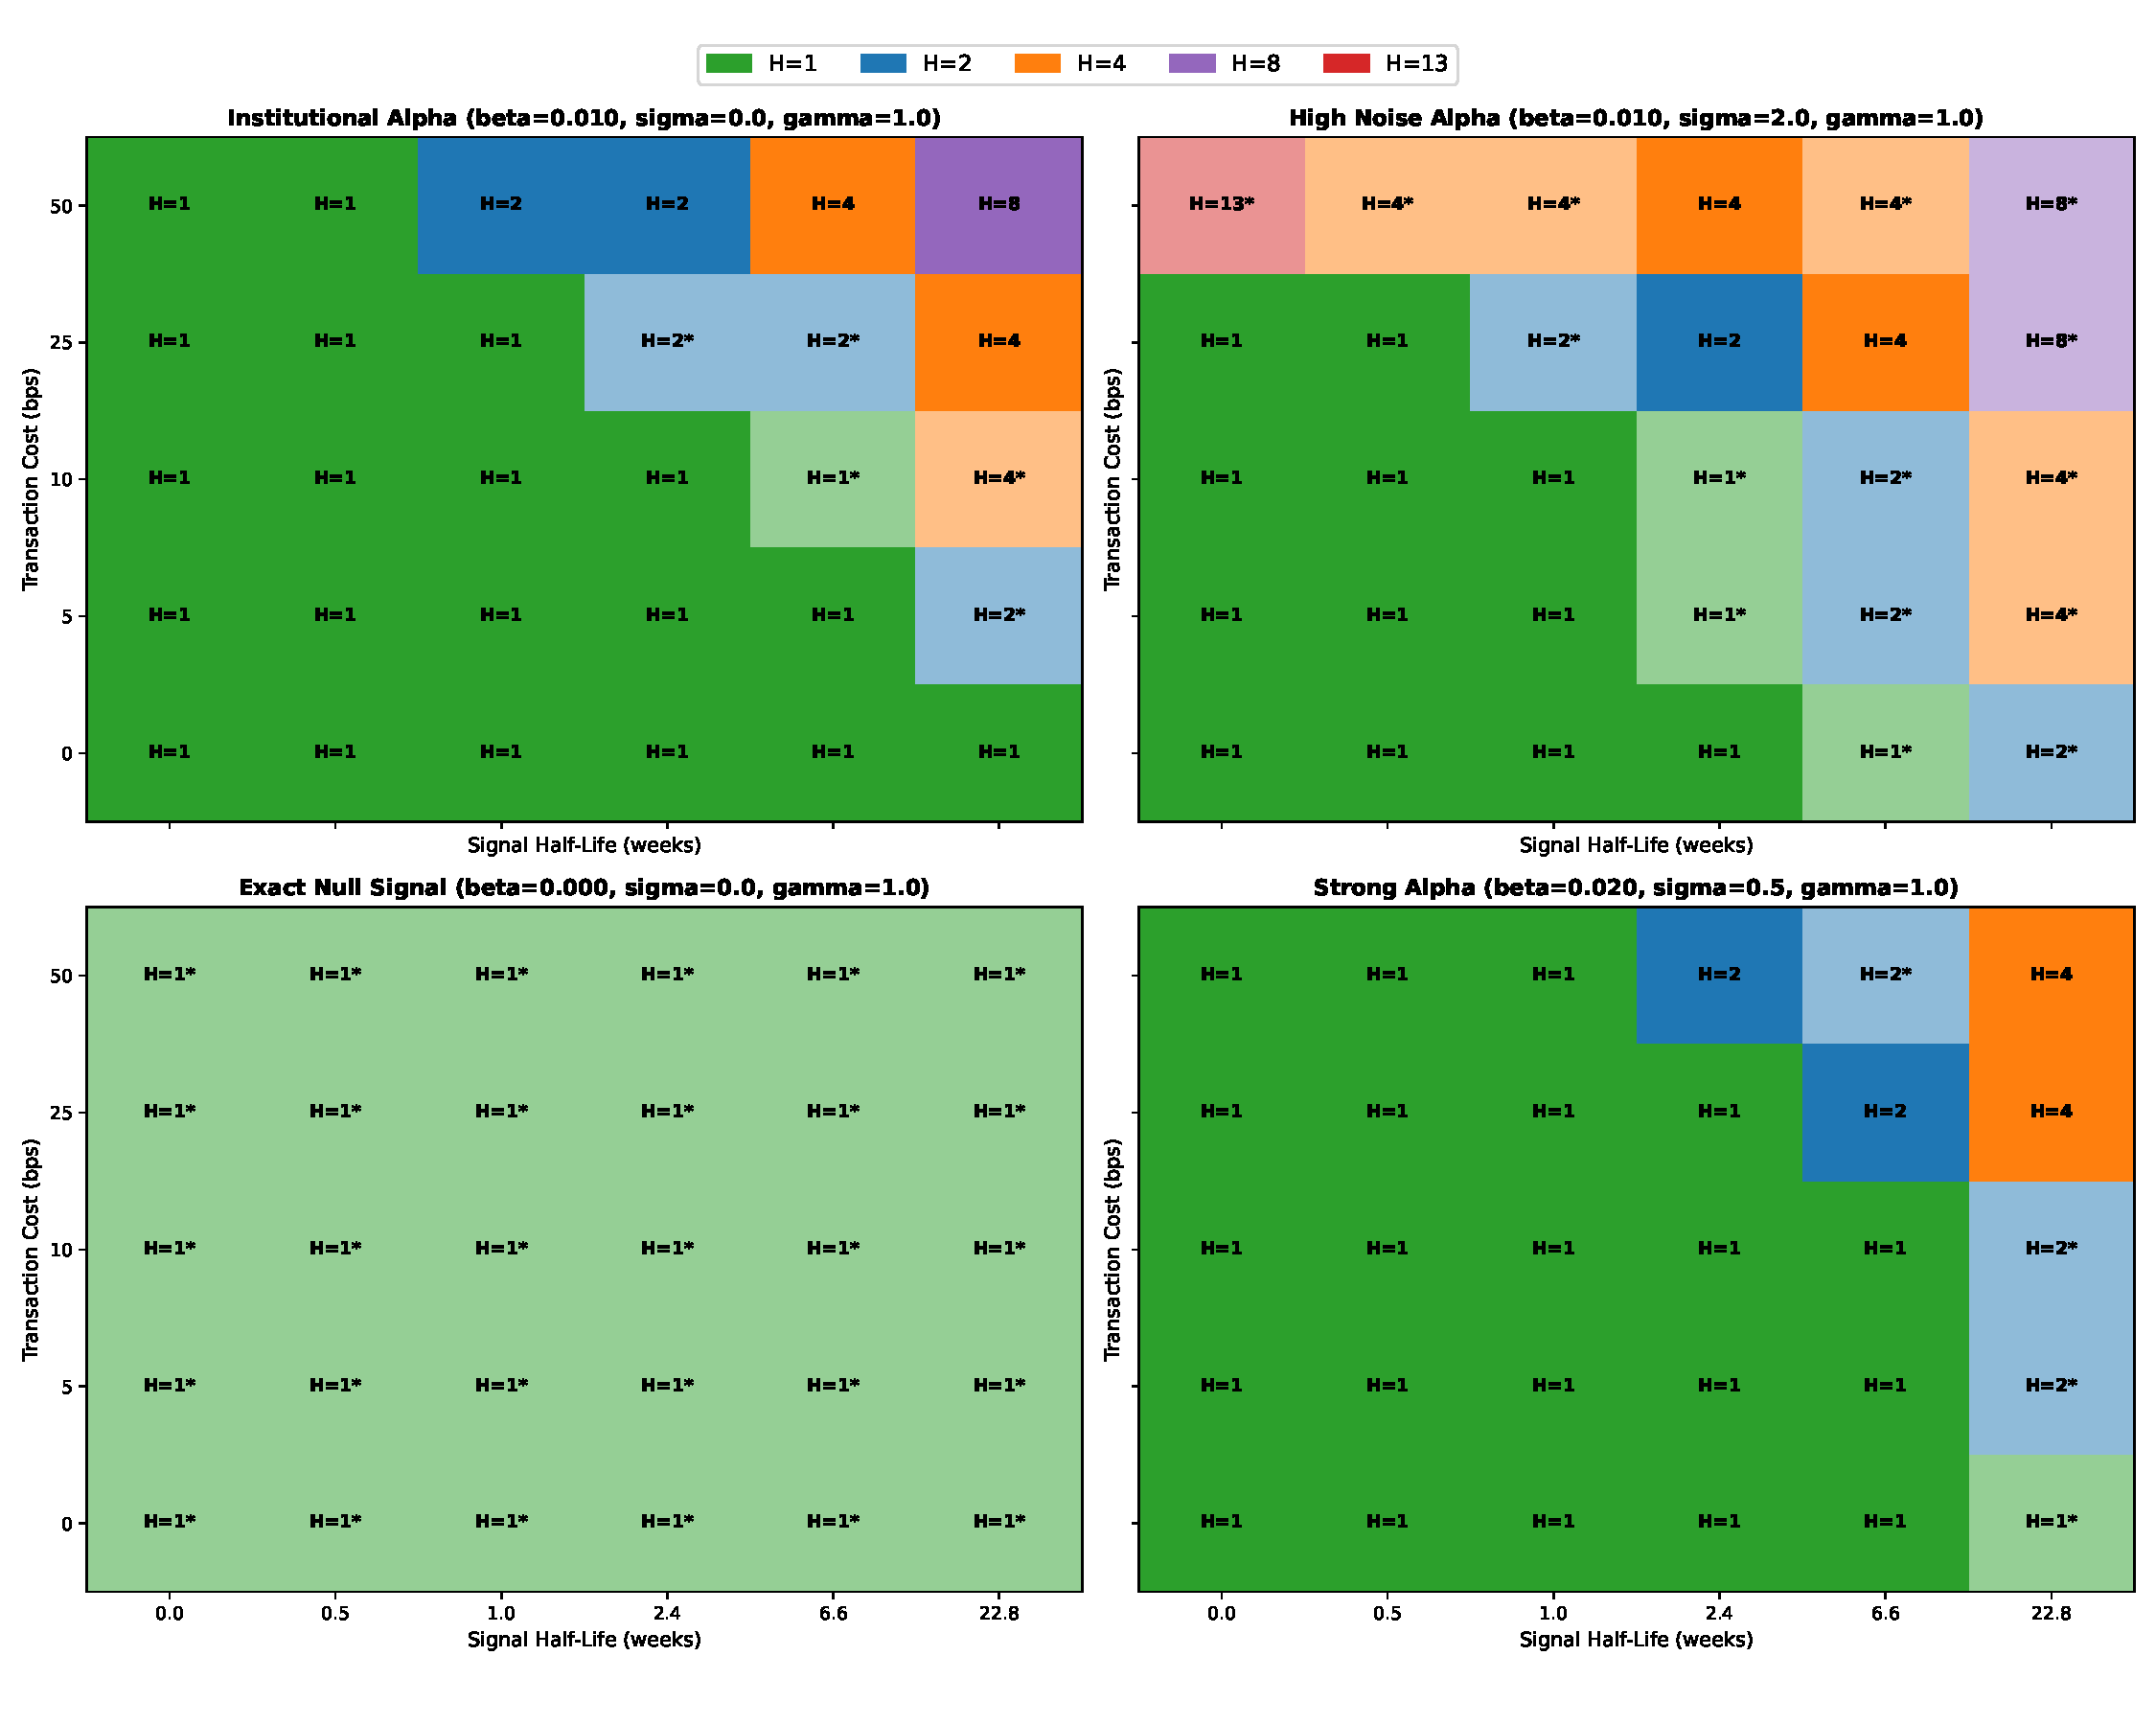
\includegraphics[width=0.95\textwidth]{figures/fig3_phase20_synthetic_horizon_frontier.pdf}
\caption{\textbf{Phase 20 Synthetic Horizon Phase Diagram.} Utility-maximizing horizon $H^*$ mapped across transaction costs $c \in [0, 50]\text{ bps}$ and signal half-life $\tau_{1/2} \in [0, 23]\text{ weeks}$. Hatched markers indicate statistical tie zones ($p \ge 0.05$). This diagram represents a controlled synthetic simulation within $H \in \{1, 2, 4, 8, 13\}$, not an empirical market frontier.}
\label{fig:phase_diagram}
\end{figure}


\section{Retrospective Empirical Motivation and Stress Tests}
\label{sec:empirical}

We connect these synthetic findings back to the retrospective empirical event-risk setting that motivated this research (Table~\ref{tab:empirical_evidence} and Figure~\ref{fig:empirical}).

\begin{table}[t]
\centering
\small
\caption{\textbf{Retrospective Empirical Evidence and Stress Tests (Phases 18 \& 19).} Panel A reports clean out-of-sample portfolio revalidation on quarterly earnings events (2022--2025). Panel B reports the architecture stress test across signal regimes. The empirical evidence demonstrates that turnover reduction ($\sim 74\%$) and volatility reduction ($\sim 66\%$) are architecture-general regularizer effects that persist even under null signals, while utility gains reverse under strong synthetic alpha (Outcome D).}
\label{tab:empirical_evidence}
\resizebox{\textwidth}{!}{%
\begin{tabular}{lcccc}
\hline
\multicolumn{5}{l}{\textbf{Panel A: Clean Empirical Revalidation (Phase 18, Quarterly Earnings Holdout 2022--2025)}} \\
\hline
\textbf{Metric} & \textbf{Single Horizon ($H=1$)} & \textbf{Cohort Stacking ($H=4$)} & \textbf{Differential ($\Delta$)} & \textbf{Statistical Status} \\
\hline
Annualized Net Return & 9.24\% & 14.71\% & +5.47\% & Arithmetic mean \\
Annualized Net Volatility & 19.59\% & 6.62\% & \textbf{-66.21\%} & Diversification gain \\
Traded Risky Turnover (L1/yr) & 73.03 & 19.01 & \textbf{-73.97\%} & Cost amortization \\
Annualized Sharpe Ratio & \textbf{0.469} & \textbf{2.223} & \textbf{+1.754} & Clean revalidation \\
Maximum Drawdown & -18.77\% & -5.00\% & +13.77\% & Capital preservation \\
Mean Net Weekly Utility (bp/wk) & 14.072 & 27.876 & \textbf{+13.804} & 95\% CI: $[-54.68, +84.33]$ \\
Gross Return Contribution & --- & --- & +0.145 & Negligible alpha gain \\
Transaction Cost Savings & --- & --- & +10.387 & Primary point driver \\
Variance Term Utility Gain & --- & --- & +3.272 & Secondary point driver \\
Residual Weeks 2--4 Rank IC & --- & --- & \textbf{0.0060} & $p = 0.105$ (Insignificant) \\
\hline
\multicolumn{5}{l}{\textbf{Panel B: Architecture-General Signal Stress Test (Phase 19)}} \\
\hline
\textbf{Signal Regime} & \textbf{Traded TO Red.} & \textbf{Net Vol Red.} & \textbf{Net $\Delta U$ (bp/wk)} & \textbf{Regime Classification} \\
\hline
Clean Empirical LoRA & 73.97\% & 66.16\% & +13.80 & Retrospective empirical \\
Ticker-Risk Baseline & 73.97\% & 69.71\% & +15.63 & Historical control \\
Random Ranking Null (50 seeds) & 73.97\% & 67.10\% & \textbf{+22.53} & Rebalancing churn null \\
Constant / Equal-Weight Null & 73.97\% & 65.67\% & \textbf{+22.40} & Time-invariant control \\
Synthetic $\alpha = 0.00$ & 73.97\% & 67.35\% & +2.04 & Noise smoothing dominates \\
Synthetic $\alpha = 0.05$ & 73.97\% & 67.30\% & +0.88 & Modest stacking advantage \\
Synthetic $\alpha = 0.10$ & 73.97\% & 67.24\% & \textbf{-0.27} & \textbf{Reversal Threshold} \\
Synthetic $\alpha = 0.20$ & 73.97\% & 67.01\% & -2.52 & Instantaneous rebalancing wins \\
Synthetic $\alpha = 0.40$ & 73.97\% & 66.07\% & -7.09 & Fresh alpha preservation \\
\hline
\end{tabular}%
}
\end{table}


\begin{figure}[t]
\centering
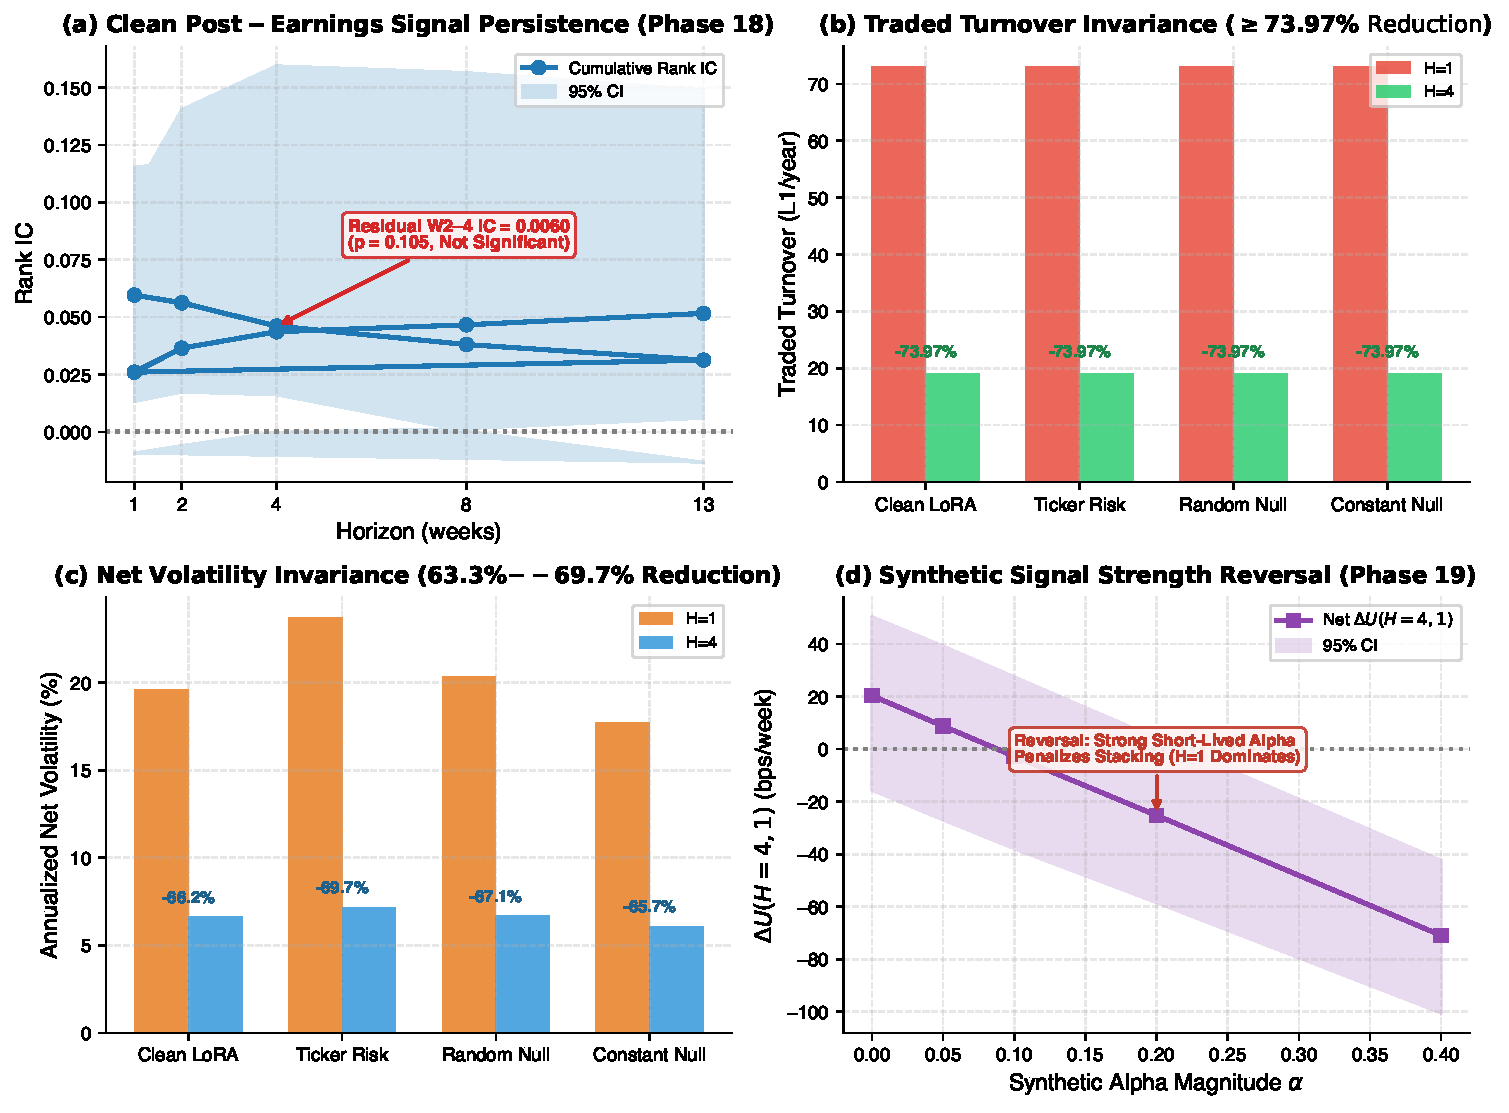
\includegraphics[width=0.95\textwidth]{figures/fig4_retrospective_empirical_motivation.pdf}
\caption{\textbf{Retrospective Empirical Motivation and Signal Stress Tests (Phases 18 \& 19).} (a) Clean signal persistence across horizons; incremental weeks 2--4 IC is statistically insignificant ($p = 0.105$). (b) Traded turnover reduction exceeds 73.97\% across empirical, null, and synthetic signals. (c) Net portfolio volatility reduction is invariant across signal quality (63.3\%--69.7\%). (d) Phase~19 synthetic signal reversal: cohort stacking delivers positive relative utility under weak/null signals, but reverses to negative relative utility under strong synthetic alpha (Outcome D).}
\label{fig:empirical}
\end{figure}

In Phase~18, clean out-of-sample revalidation of quarterly post-earnings portfolios on uncompromised metadata exhibited:
\begin{itemize}
    \item Annualized net return: $9.24\%$ ($H=1$) vs $14.71\%$ ($H=4$)
    \item Annualized net volatility: $19.59\%$ ($H=1$) vs $6.62\%$ ($H=4$) ($-66.21\%$ reduction)
    \item Annualized traded risky turnover: $73.03$ ($H=1$) vs $19.01$ ($H=4$) ($-73.97\%$ reduction)
    \item Annualized Sharpe ratio: \textbf{$0.469$} ($H=1$) to \textbf{$2.223$} ($H=4$)
    \item Incremental weeks 2--4 predictive persistence: Rank IC $= 0.0060$, $p = 0.105$ (insignificant)
    \item Point utility attribution: Gross return $\Delta = +0.15\text{ bp/wk}$, Cost saving $= +10.39\text{ bp/wk}$, Variance gain $= +3.27\text{ bp/wk}$
\end{itemize}

When these empirical parameters ($c = 10\text{ bps}$, $\gamma = 1.0$, $\beta \in [0.005, 0.010]$, $\sigma_{\text{noise}} \in [1.0, 2.0]$, $\rho \in [0.50, 0.75]$) are mapped into the Phase~20 synthetic simulation grid, the simulated utility-maximizing horizon lies at $H^* \in \{1, 2\}$ under continuous asset dynamics, shifting to $H=4$ and $H=8$ as transaction costs rise to $25\text{--}50\text{ bps}$ or noise increases.

Why, then, did the empirical earnings strategy strongly favor $H=4$? The explanation lies in \textbf{panel churn}: because corporate earnings announcements occur quarterly, the weekly cross-section of reporting companies was 100\% disjoint from week to week. Under un-stacked rebalancing ($H=1$), this disjointness forced an extreme baseline turnover of $\sim 72\text{--}104\text{x/year}$. Multiplying baseline turnover $\text{TO}_0$ by a factor of 3 to 4 increases the marginal economic value of cost amortization proportionally, shifting the effective operating horizon directly to $H=4$.

Furthermore, Phase~19 stress-testing proved that turnover ($-73.97\%$) and volatility ($-66.2\%$) reductions were architecture-general, persisting across random-ranking and constant controls. Crucially, Phase~19 revealed a directional reversal: stacking was most advantageous under weak or null signals, but lost advantage under strong synthetic alpha ($\alpha \ge 0.10$, Outcome D). The synthetic simulation provides the unified mechanistic explanation: \textbf{cohort stacking survived as an architectural regularizer, not as an alpha-capture mechanism}.


\section{Negative-Result Provenance and Falsification Summary}
\label{sec:provenance}

For scientific transparency, we document how earlier candidate hypotheses were systematically investigated and falsified across the research trajectory:
\begin{enumerate}
    \item \textbf{Bayesian Epistemic Uncertainty (Phases 11--16.1)}: Evaluated as an asset-selection and market-timing signal. Forensic audits revealed target outcome leakage (`\texttt{move\_1d}' in training text) that artificially inflated validation AUROC ($>0.999$). Furthermore, the apparent correlation between predictive entropy and absolute prediction error ($\rho \approx 0.60$) was mathematically proven to be an algebraic artifact of 80/20 class imbalance under probability shrinkage, mechanically forcing within-class rank correlations to $\pm 1.0000$. Clean retraining showed that Bayesian LoRA ($\text{Brier} = 0.15987$) was matched by deterministic LoRA ($0.16079$) and a constant base-rate null ($0.16000$), while 32-draw Monte Carlo sampling imposed a $30\times$ latency penalty over a single deterministic forward pass of the posterior mean.
    \item \textbf{Collaborative LoRA Specialist Weighting (Pilot)}: Evaluated cross-sector specialization with learned coordination weights. Learned weights degenerated to a single specialist, failing continuation criteria.
    \item \textbf{Prospective 2026 Confirmation (Phase 10)}: Provenance audits verified that all historical equity returns terminated on May 15, 2025. In adherence to non-manufacturing protocols, prospective claims were retracted and classified under retrospective holdout scope.
\end{enumerate}


\section{Limitations and Boundary Conditions}
\label{sec:limitations}

We explicitly articulate ten boundary conditions governing this study:
\begin{enumerate}
    \item \textbf{Controlled Synthetic Environment}: Phase~20 findings are established in a controlled simulation and require empirical verification in specific asset classes.
    \item \textbf{Linear-Gaussian Signal Decay}: Latent factors follow stationary AR(1) dynamics; real markets exhibit non-linear regime shifts, jumps, and structural breaks.
    \item \textbf{Linear Transaction Friction}: Costs are modeled proportionally ($c \cdot \text{TO}$); institutional execution involves square-root price impact and temporary liquidity depletion.
    \item \textbf{No Liquidity or Capacity Constraints}: The model assumes unlimited liquidity at cost $c$; capacity limits would penalize high-turnover short horizons even more severely.
    \item \textbf{Static Holding Horizons}: $H$ is held constant over the portfolio lifecycle; adaptive, volatility-conditioned horizons are left for future research.
    \item \textbf{Discrete Candidate Grid}: Optimization is performed over the frozen grid $H \in \{1, 2, 4, 8, 13\}$ rather than continuous holding periods.
    \item \textbf{Finite-Memory Truncation}: Truncating latent history at $K = 52$ calendar weeks captures $\approx 80\%$ of asymptotic signal weight for $\rho = 0.97$ ($0.97^{52} \approx 0.2032$), representing an explicitly finite-memory approximation.
    \item \textbf{Reconstructed Historical Returns}: Phase~18 used geometrically interpolated event-endpoint returns, which mechanically smooth intraweek price volatility.
    \item \textbf{Retrospective Data Only}: All empirical analyses terminated on May 15, 2025; no independent prospective data exists in the repository.
    \item \textbf{Absence of Live Execution}: Backtests omit borrow availability, short rebate rates, exchange fee tiers, and real-time execution slippage.
\end{enumerate}


\section{Conclusion and Practical Design Principles}
\label{sec:conclusion}

Overlapping cohort portfolios are not an empirical heuristic for capturing prolonged price drift; they are a formal \textbf{temporal regularization mechanism}. By pooling staggered sub-portfolios across time, cohort stacking trades responsiveness to fresh signals against execution turnover and estimation noise.

For quantitative portfolio managers, our findings establish clear architectural design principles:
\begin{itemize}
    \item \textbf{Measure Signal Half-Life Before Setting Horizons}: For transient signals ($\tau_{1/2} < 0.5\text{ weeks}$), stacking beyond $H=1$ severely penalizes performance unless transaction costs exceed $25\text{ bps}$.
    \item \textbf{Use Stacking to Dampen High-Frequency Panel Churn}: In event-driven strategies with disjoint cross-sections (e.g., quarterly earnings), cohort stacking is an indispensable structural dampener that reduces turnover by $50\text{--}75\%$.
    \item \textbf{Recognize the Friction-Decay Frontier}: The utility-maximizing horizon increases monotonically with transaction costs, signal half-life, observation noise, and risk aversion. When alpha is scarce and noisy, temporal regularization is often the single most impactful lever for institutional portfolio implementation.
\end{itemize}


\section*{Data and Code Availability}
Code, preregistration protocols, simulation specifications, and derived research artifacts supporting the findings of this study are available in the project repository. Historical empirical inputs are subject to third-party licensing constraints documented in the repository. The Phase~20 controlled synthetic simulation is fully reproducible from the frozen configuration and random seed schedule ($S \in \{200001, \dots, 200030\}$).

\section*{Declarations}
The authors declare that they have no known competing financial interests or personal relationships that could have appeared to influence the work reported in this paper.

\bibliographystyle{plainnat}
\bibliography{references}

\end{document}
